\documentclass[a4paper,11pt]{article}
\usepackage[utf8]{inputenc}
\usepackage{amsmath}
\usepackage{amsfonts}
\usepackage{amssymb}
\usepackage{graphicx}
\usepackage{tabularx}
\usepackage[font=scriptsize]{caption}
\usepackage[font=scriptsize]{subcaption}
\usepackage{wrapfig}
\usepackage[backend=biber]{biblatex}

\addbibresource{nn.bib}
\renewcommand\thesubsection{\alph{subsection}}


%opening
\title{A population firing rate encoder based on cortical minicolumns}
\author{Vince Baker, advisor: Dr. Luis Cruz Cruz\\ Drexel University Department of Physics}

\begin{document}

\maketitle

\begin{abstract}
We propose a neural circuit topology to encode population firing rate information.
The topology is based on the observed minicolumn structure found in the mammalian cortex.
The proposed neural circuit provides a strong, sparse encoding of peaks in the population firing rate through synchronized traveling waves in the minicolumn structures.
\end{abstract}

\section{Introduction} 
Information in the brain is encoded by the firing rates of neurons.
Individual neurons in the brain do not reliably respond to a specific stimulus in a consistent manner.
A stimulus may, however, be reliably encoded in the average firing rate of a pool of neurons with similar tuning \cite{trappenberg}.

The mammalian cortex has a laminar structure segmented into layers \cite{banich}.
Perpendicular to these layers are vertical units of organization called minicolumns or microcolumns that travers layers II through VI \cite{buxhoeveden2002}\cite{cruz2005}.
These minicolumns are about 30-50 $\mu$m wide and contain about 100 neurons.
Although this minicolumn organization was observed decades ago the functional purpose of minicolumns, if any, remains unclear \cite{horton2005}.

Neurons in the cortex are dominated by local connectivity, such that neurons are most strongly connected to nearby neurons \cite{levy2012}.
Locally connected neurons can spread their firings to neighboring neurons creating what has been called a travelling wave of neuron activation. 
These travelling waves in locally connected networks have been observed in the cortex of mammalian brains as well as in vitro, and subsequently have been reproduced in silico \cite{keane2015}\cite{ermentrout2001}\cite{wu2008}.
Cortical traveling waves have been observed on multiple spatial and temporal scales, and a number of functional roles have been proposed \cite{muller2018}.

We propose a neural circuit to encode the average firing rate of a pool of neurons.
The proposed circuit is composed of locally connected neurons arranged in minicolumns.
A pool of input neurons is connected to the base of the minicolumns.
Peaks in the population firing rate of the input pool evoke traveling waves that travel up the minicolumns.
These traveling waves produce a strong, sparse representation at the top of the minicolumns.
We observe that weakly connected minicolumns produce the most reliable, clean and efficient encoding.

\section{Methods}
Neuron and synapse dynamics, single column model
\\ \\
Minicolumn ensembles (one big column, weakly connected columns, disconnected minicolumns)
\\ \\
The input to our system is generated from a pool of 50 neurons.
Each input neuron is connected to every excitatory neuron at the base layer of the minicolumn ensemble with a probability of connection of $50\%$ and a connection strength of $5/2$. 
The input neurons have a common firing rate that varies over time.
For each $10 ms$ time window a Poisson spike train of duration $10 ms$ is generated for every input neuron based on the instantaneous firing rate.
The output from each neuron in the input pool is calculated by convolving the neuron's spike train with an exponential synaptic response $e^{(t-t^f)/\sigma}$ where $t^f$ is the neuron firing time and $\sigma = 4ms$.
The input signal to each neuron in the base layer of the minicolumn ensemble is summed from the input pool stimulus according to the synaptic connections (Figure \ref{fig:firingrate_input}).

\begin{figure}[!htb]
 \caption{Firing rate input. The instantaneous firing rate (top) is encoded into spike trains of a pool of 50 neurons (middle), generating a stimulus to the base layer of the minicolumn ensemble (bottom). The stimulus at the bottom is shown as a membane potential in Volts.}
 \label{fig:firingrate_input}
 \centering
   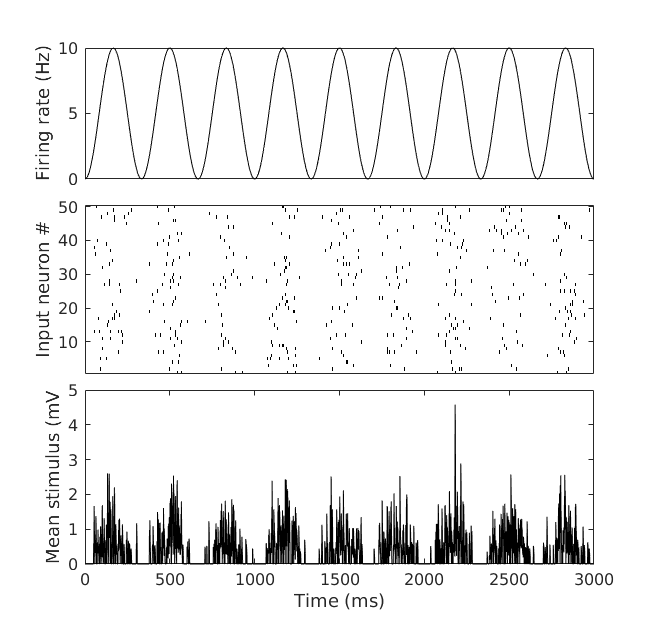
\includegraphics[width=0.5\textwidth]{fig/InputFiringRate}
\end{figure}

We measure the output as the average membrane potential of the neurons in the top layer of the minicolumn ensemble.
We characterize the quality of the firing rate encoding by the correlation between the output potential and the instantaneous firing rate.
We also measure 


Output characterization
-Correlation
-Noise
-Sparsity
-Efficiency of column ensemble

\section{Results}

\begin{figure}[!htb]
 \caption{Firing rate encoding example. The instantaneous firing rate (top) is shown with the mean membrane potential of the input layer (middle) and the output layer (bottom). The output layer shows a cleaner signal with stronger spikes.}
 \label{fig:firingrate_example}
 \centering
   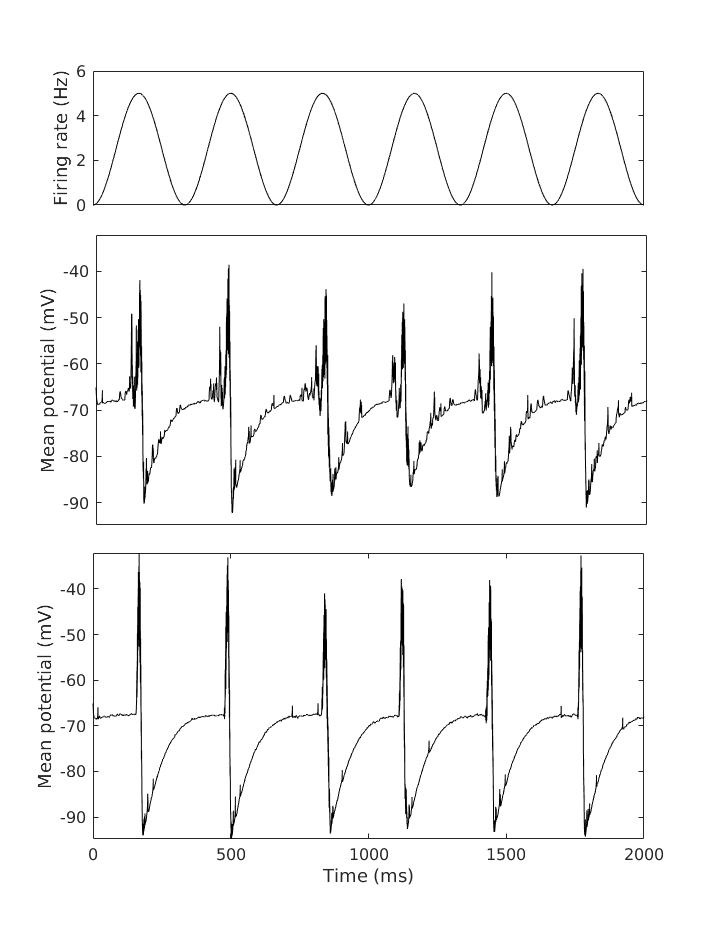
\includegraphics[width=0.5\textwidth]{fig/FiringRateEncodingExample}
\end{figure}

\section{Discussion}


\clearpage
\printbibliography

\end{document}
